
%(BEGIN_QUESTION)
% Copyright 2012, Tony R. Kuphaldt, released under the Creative Commons Attribution License (v 1.0)
% This means you may do almost anything with this work of mine, so long as you give me proper credit

Tolk trykkmålingen som vises av dette manometeret, forutsatt en nøyaktighet på $\pm$ 2\% av full skala:

$$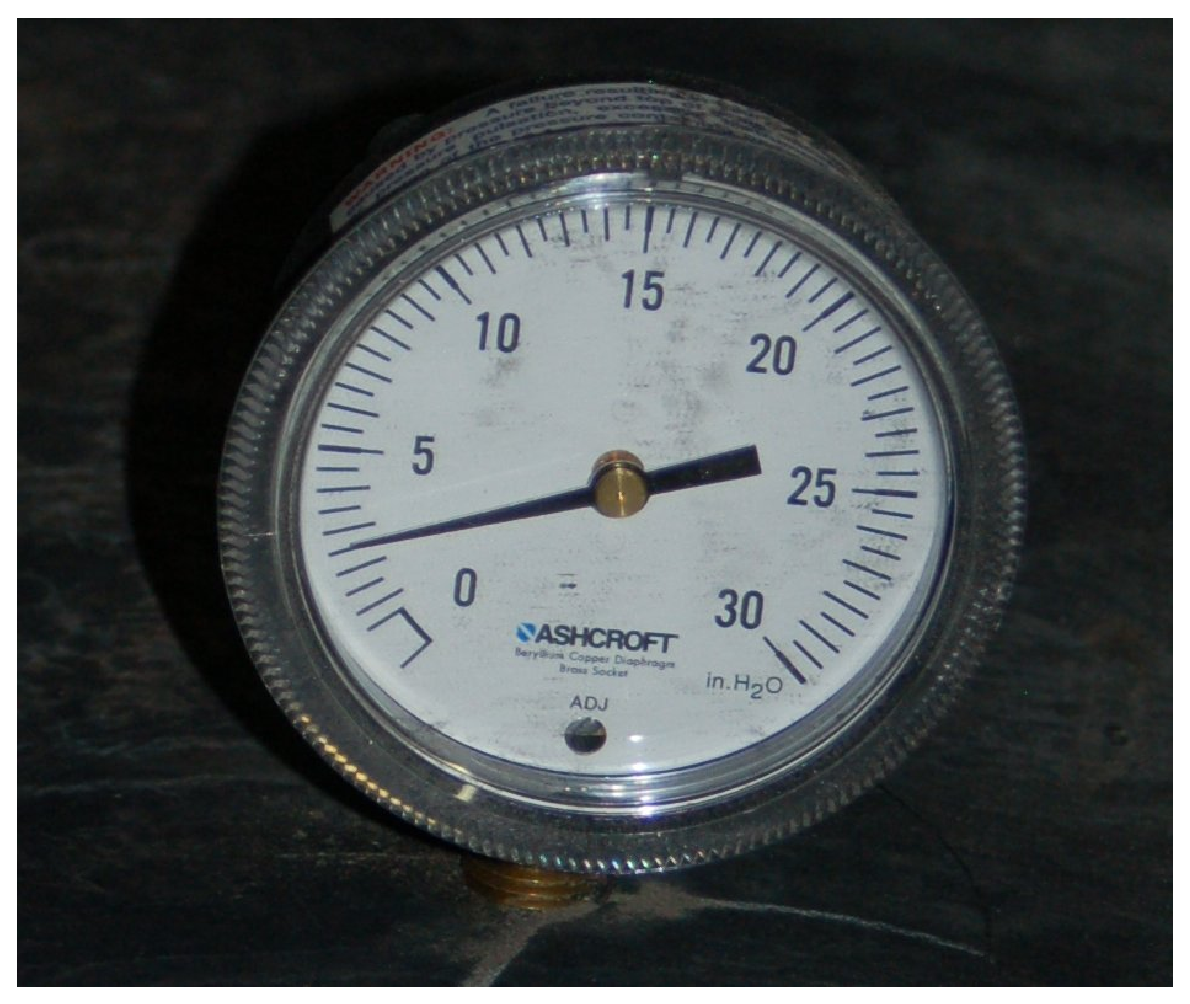
\includegraphics[width=15.5cm]{i01155x01.eps}$$

Hvor lavt og hvor høyt kan trykket faktisk være, gitt oppgitt nøyaktighet for dette manometeret?

\underbar{file i01155}
%(END_QUESTION)





%(BEGIN_ANSWER)

Trykk = 2.5 "H$_{2}$O $\pm$ 0.6 "H$_{2}$O.  Det betyr at det faktiske trykket kan være så lavt som 1.9 "H$_{2}$O eller så høyt som 3.1 "H$_{2}$O.

 
\vskip 10pt

Hvis du ser nøye på bildet, ser du at kameraets vinkel mot manometerskalaen ikke er rett på. Derfor vil avlesningen få en viss {\it parallaksefeil}.  Hvis kameraet hadde stått lavere og mer rett foran skalaen, kunne vi kanskje sett nålen peke mellom 2.5 og 3, noe som ville gitt et trykk på 2.75 "H$_{2}$O $\pm$0.6 "H$_{2}$O.

%(END_ANSWER)





%(BEGIN_NOTES)


%INDEX% Measurement, analog gauge reading

%(END_NOTES)

